\iffalse
This file is protected by Copyright. Please refer to the COPYRIGHT file
distributed with this source distribution.

This file is part of OpenCPI <http://www.opencpi.org>

OpenCPI is free software: you can redistribute it and/or modify it under the
terms of the GNU Lesser General Public License as published by the Free Software
Foundation, either version 3 of the License, or (at your option) any later
version.

OpenCPI is distributed in the hope that it will be useful, but WITHOUT ANY
WARRANTY; without even the implied warranty of MERCHANTABILITY or FITNESS FOR A
PARTICULAR PURPOSE. See the GNU Lesser General Public License for more details.

You should have received a copy of the GNU Lesser General Public License along
with this program. If not, see <http://www.gnu.org/licenses/>.
\fi

%----------------------------------------------------------------------------------------
% Required document specific properties
%----------------------------------------------------------------------------------------
\def\comp{capture\_{}v2}
\edef\ecomp{capture_v2}
\def\Comp{Capture v2}
\def\docTitle{\Comp{} Component Data Sheet}
\def\snippetpath{../../../../../../doc/av/tex/snippets}
%----------------------------------------------------------------------------------------
% Global latex header (this must be after document specific properties)
%----------------------------------------------------------------------------------------
\iffalse
This file is protected by Copyright. Please refer to the COPYRIGHT file
distributed with this source distribution.

This file is part of OpenCPI <http://www.opencpi.org>

OpenCPI is free software: you can redistribute it and/or modify it under the
terms of the GNU Lesser General Public License as published by the Free Software
Foundation, either version 3 of the License, or (at your option) any later
version.

OpenCPI is distributed in the hope that it will be useful, but WITHOUT ANY
WARRANTY; without even the implied warranty of MERCHANTABILITY or FITNESS FOR A
PARTICULAR PURPOSE. See the GNU Lesser General Public License for more details.

You should have received a copy of the GNU Lesser General Public License along
with this program. If not, see <http://www.gnu.org/licenses/>.
\fi

% Sets OpenCPI Version used throughout all the docs. This is updated by
% scripts/update-release.sh when a release is being made and must not
% be changed manually.
\def\ocpiversion{v2.2.0}

\documentclass{article}
\author{}  % Force author to be blank
\date{OpenCPI Release:\ \ \ocpiversion}  % Force date to be blank and override date with version
\title{OpenCPI\\\docTitle}  % docTitle must be defined before including this file
%----------------------------------------------------------------------------------------
% Paper size, orientation and margins
%----------------------------------------------------------------------------------------
\usepackage{geometry}
\geometry{
  letterpaper,  % paper type
  portrait,     % text direction
  left=.75in,   % left margin
  top=.75in,    % top margin
  right=.75in,  % right margin
  bottom=.75in  % bottom margin
}
%----------------------------------------------------------------------------------------
% Header/Footer
%----------------------------------------------------------------------------------------
\usepackage{fancyhdr} \pagestyle{fancy}  % required for fancy headers
\renewcommand{\headrulewidth}{0.5pt}
\renewcommand{\footrulewidth}{0.5pt}
\lhead{\small{\docTitle}}
\rhead{\small{OpenCPI}}
%----------------------------------------------------------------------------------------
% Various packages
%----------------------------------------------------------------------------------------
\usepackage{amsmath}
\usepackage[page,toc]{appendix}  % for appendix stuff
\usepackage{enumitem}
\usepackage{graphicx}   % for including pictures by file
\usepackage{hyperref}   % for linking urls and lists
\usepackage{listings}   % for coding language styles
\usepackage{pdflscape}  % for landscape view
\usepackage{pifont}     % for sideways table
\usepackage{ragged2e}   % for justify
\usepackage{rotating}   % for sideways table
\usepackage{scrextend}
\usepackage{setspace}
\usepackage{subfig}
\usepackage{textcomp}
\usepackage[dvipsnames,usenames]{xcolor}  % for color names see https://en.wikibooks.org/wiki/LaTeX/Colors
\usepackage{xstring}
\uchyph=0  % Never hyphenate acronyms like RCC
\renewcommand\_{\textunderscore\allowbreak}  % Allow words to break/newline on underscores
%----------------------------------------------------------------------------------------
% Table packages
%----------------------------------------------------------------------------------------
\usepackage[tableposition=top]{caption}
\usepackage{float}
\floatstyle{plaintop}
\usepackage{longtable}  % for long possibly multi-page tables
\usepackage{multicol}   % for more advanced table layout
\usepackage{multirow}   % for more advanced table layout
\usepackage{tabularx}   % c=center,l=left,r=right,X=fill
% These define tabularx columns "C" and "R" to match "X" but center/right aligned
\newcolumntype{C}{>{\centering\arraybackslash}X}
\newcolumntype{M}[1]{>{\centering\arraybackslash}m{#1}}
\newcolumntype{P}[1]{>{\centering\arraybackslash}p{#1}}
\newcolumntype{R}{>{\raggedleft\arraybackslash}X}
%----------------------------------------------------------------------------------------
% Block Diagram / FSM Drawings
%----------------------------------------------------------------------------------------
\usepackage{tikz}
\usetikzlibrary{arrows,decorations.markings,fit,positioning,shapes}
\usetikzlibrary{automata}  % used for the fsm
\usetikzlibrary{calc}      % for duplicating clients
\usepgfmodule{oo}          % to define a client box
%----------------------------------------------------------------------------------------
% Colors Used
%----------------------------------------------------------------------------------------
\usepackage{colortbl}
\definecolor{blue}{rgb}{.7,.8,.9}
\definecolor{ceruleanblue}{rgb}{0.16, 0.32, 0.75}
\definecolor{cyan}{rgb}{0.0,0.6,0.6}
\definecolor{darkgreen}{rgb}{0,0.6,0}
\definecolor{deepmagenta}{rgb}{0.8, 0.0, 0.8}
\definecolor{maroon}{rgb}{0.5,0,0}
%----------------------------------------------------------------------------------------
% Define where to hyphenate
%----------------------------------------------------------------------------------------
\hyphenation{Cent-OS}
\hyphenation{install-ation}
%----------------------------------------------------------------------------------------
% Define Commands & Rename Commands
%----------------------------------------------------------------------------------------
\newcommand{\code}[1]{\texttt{#1}}  % For inline code snippet or command line
\newcommand{\sref}[1]{Section~\ref{#1}}  % To quickly reference a section
\newcommand{\todo}[1]{\textcolor{red}{TODO: #1}\PackageWarning{TODO:}{#1}}  % To do notes
\renewcommand{\contentsname}{Table of Contents}
\renewcommand{\listfigurename}{List of Figures}
\renewcommand{\listtablename}{List of Tables}

% This gives a link to gitlab.io document. By default, it outputs the filename.
% You can optionally change the link, e.g.
% \githubio{FPGA\_Vendor\_Tools\_Installation\_Guide.pdf} vs.
% \githubio[\textit{FPGA Vendor Tools Installation Guide}]{FPGA\_Vendor\_Tools\_Installation\_Guide.pdf}
% or if you want the raw ugly URL to come out, \githubioURL{FPGA_Vendor_Tools_Installation_Guide.pdf}
\newcommand{\githubio}[2][]{% The default is for FIRST param!
\href{http://opencpi.gitlab.io/releases/\ocpiversion/docs/#2}{\ifthenelse{\equal{#1}{}}{\texttt{#2}}{#1}}}
\newcommand{\gitlabcom}[2][]{% The default is for FIRST param!
\href{http://gitlab.com/opencpi/#2}{\ifthenelse{\equal{#1}{}}{\texttt{#2}}{#1}}}
\newcommand{\githubioURL}[1]{\url{http://opencpi.gitlab.io/releases/\ocpiversion/docs/#1}}
% Lastly, if you want a SINGLE leading path stripped, e.g. assets/X.pdf => X.pdf:
\newcommand{\githubioFlat}[1]{%
\StrBehind{#1}{/}[\den]%
\href{http://opencpi.gitlab.io/releases/\ocpiversion/docs/#1}{\texttt{\den}}%
}
%----------------------------------------------------------------------------------------
% VHDL Coding Language Style
% modified from: http://latex-community.org/forum/viewtopic.php?f=44&t=22076
%----------------------------------------------------------------------------------------
\lstdefinelanguage{VHDL}
{
  basicstyle=\ttfamily\footnotesize,
  columns=fullflexible,keepspaces,  % https://tex.stackexchange.com/a/46695/87531
  keywordstyle=\color{ceruleanblue},
  commentstyle=\color{darkgreen},
  morekeywords={
    library, use, all, entity, is, port, in, out, end, architecture, of,
    begin, and, signal, when, if, else, process, end,
  },
  morecomment=[l]--
}
%----------------------------------------------------------------------------------------
% XML Coding Language Style
% modified from http://tex.stackexchange.com/questions/10255/xml-syntax-highlighting
%----------------------------------------------------------------------------------------
\lstdefinelanguage{XML}
{
  basicstyle=\ttfamily\footnotesize,
  columns=fullflexible,keepspaces,
  morestring=[s]{"}{"},
  morecomment=[s]{!--}{--},
  commentstyle=\color{darkgreen},
  moredelim=[s][\color{black}]{>}{<},
  moredelim=[s][\color{cyan}]{\ }{=},
  stringstyle=\color{maroon},
  identifierstyle=\color{ceruleanblue}
}
%----------------------------------------------------------------------------------------
% DIFF Coding Language Style
% modified from http://tex.stackexchange.com/questions/50176/highlighting-a-diff-file
%----------------------------------------------------------------------------------------
\lstdefinelanguage{diff}
{
  basicstyle=\ttfamily\footnotesize,
  columns=fullflexible,keepspaces,
  breaklines=true,                            % wrap text
  morecomment=[f][\color{ceruleanblue}]{@@},  % group identifier
  morecomment=[f][\color{red}]-,              % deleted lines
  morecomment=[f][\color{darkgreen}]+,        % added lines
  morecomment=[f][\color{deepmagenta}]{---},  % Diff header lines (must appear after +,-)
  morecomment=[f][\color{deepmagenta}]{+++},
}
%----------------------------------------------------------------------------------------
% Python Coding Language Style
%----------------------------------------------------------------------------------------
\lstdefinelanguage{python}
{
  basicstyle=\ttfamily\footnotesize,
  columns=fullflexible,keepspaces,
  keywordstyle=\color{ceruleanblue},
  commentstyle=\color{darkgreen},
  stringstyle=\color{orange},
  morekeywords={
    print, if, sys, len, from, import, as, open,close, def, main, for, else,
    write, read, range,
  },
  comment=[l]{\#}
}
%----------------------------------------------------------------------------------------
% Fontsize Notes in order from smallest to largest
%----------------------------------------------------------------------------------------
%    \tiny
%    \scriptsize
%    \footnotesize
%    \small
%    \normalsize
%    \large
%    \Large
%    \LARGE
%    \huge
%    \Huge

%----------------------------------------------------------------------------------------

\begin{document}
\maketitle
\thispagestyle{empty}
\newpage

\begin{center}
	\textit{\textbf{Revision History}}
	\begin{table}[H]
		\label{table:revisions} % Add "[H]" to force placement of table
		\begin{tabularx}{\textwidth}{|c|X|l|}
			\hline
			\rowcolor{blue}
			\textbf{Revision} & \textbf{Description of Change} & \textbf{Date} \\
		    \hline
		    v1.4 & Initial Release & 10/2018 \\
		    \hline
            v1.5 & Version bump. & 4/2019 \\
		    \hline
		     v1.6 & Converted Worker to version 2 & 11/2019 \\
		    \hline
		    v1.7 & Table of Worker Configurations and Resource Utilization Table removed & 5/2020 \\
			\hline
		\end{tabularx}
	\end{table}
\end{center}
\newpage

\def\name{\comp}
\def\workertype{}
\def\version{\ocpiversion}
\def\releasedate{11/2019}
\def\componentlibrary{ocpi.assets.util\_{}comps}
\def\workers{\comp{}.hdl}
\def\testedplatforms{isim, Matchstiq-Z1(PL), xsim, ZedBoard(PL)}
\section*{Summary - \Comp}
\begin{tabular}{|c|M{13.5cm}|}
  \hline
  \rowcolor{blue}
   & \\
  \hline
  Name              & \comp             \\
  \hline
  Worker Type       & \workertype       \\
  \hline
  OpenCPI Release   & \ocpiversion      \\
  \hline
  Last Update       & \releasedate      \\
  \hline
  Component Library & \componentlibrary \\
  \hline
  Workers           & \workers          \\
  \hline
  Tested Platforms  & \testedplatforms  \\
  \hline
\end{tabular}


\section*{Functionality}
\begin{flushleft}

The {\comp} component provides the ability to store an input port's
data. Two modes are supported: \newline
* 'leading' - capture all messages from input port until the buffer is full. This has the affect of capturing messages from the start of an application. \newline
* 'trailing' - capture all messages from input port and allow the buffer's content to be overwritten while application is in operation. This has the affect of capturing all messages (a buffers worth) near the end of an application. \newline

This component provides an optional output port, so that, it may be
placed between two components. The input messages are directly passed to
the output port with a latency of the control plane clock cycles. \newline

The {\comp} component takes input port messages and stores their data in a buffer via the \texttt{data} property as 4 byte words. Metadata associated with each message is stored as a record in a metadata buffer via the \texttt{metadata} property. It captures four 4 byte words of metadata. The first metadata word is the opcode of the message and message size (bytes); opcode 8 MSB and message size 24 LSB. The second word is the fraction time stamp for the EOM. The third word is the fraction time stamp for the SOM. And the fourth word is the seconds timestamp for the SOM. So that the metadata can be read on a little-endian processor, the ordering of the metadata is as follows: \newline

1) opcode (8-bit) \& message size (24-bit), \\
2) eom fraction (32-bit), \\
3) som fraction (32-bit), \\
4) som seconds (32-bit) \newline

Some example python code for reading in the \texttt{metadata} property values written to a file packed little-endian:
    \begin{lstlisting}[language=Python]
    data = struct.unpack('<I', ifile.read(4))[0] # 32/8 = 4 bytes
    \end{lstlisting}


When the number of bytes sent for a message is not a multiple of 4, only the
last (number of bytes modulus 4) least significant bytes of the last word
in the data buffer represent received data. The (number of bytes modulus 4)
most significant bytes will always be zero in the last word in the data
buffer. \\
For example, given that last captured data buffer word is 0x0000005a: \newline
- if number of bytes is 5, the last data received was 0x5a. \\
- if number of bytes is 6, the last data received was 0x005a. \newline


The {\comp} component counts the number of metadata records (\texttt{metadataCount}) have been captured and how many data words have been captured (\texttt{dataCount}). It allows for the option to wrap around and continue to capture data and metadata once the buffers are full or to stop capturing data and metadata when the data and metadata buffers are full via the stoponFull property. \newline

When \texttt{stopOnFull} is true (leading), data and metadata will be captured as long as the metadata buffer is not full. The data buffer will loop if it is not full and the metadata buffer is not full. The metadata buffer will loop independently until it is not full. When \texttt{stopOnFull} is false (trailing), the data and metadata buffers loop independently. There will be a wrap around when the data and metadata buffers are full and data and metadata will continue to be captured.  \newline

The component also has properties that keep track of whether or not the metadata and data buffers are full; \texttt{metaFull} and \texttt{dataFull}. \newline

\end{flushleft}

\section*{Block Diagrams}
	\subsection*{Top level}
\begin{center}
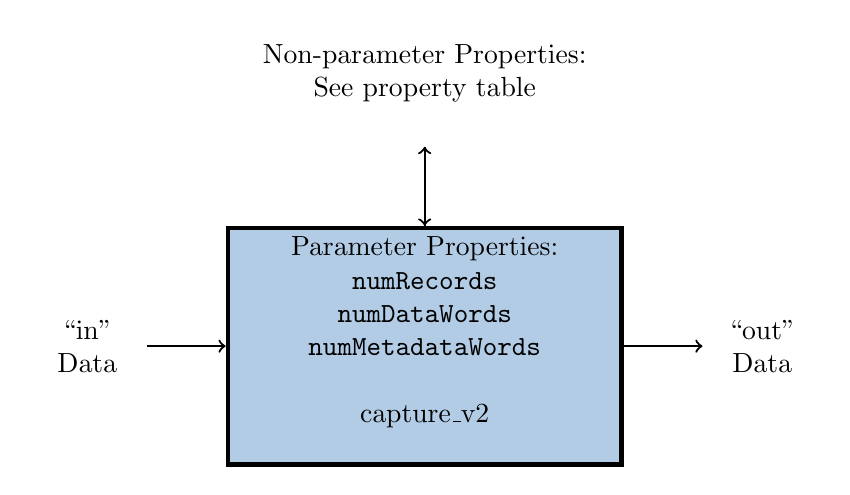
\begin{tikzpicture}[% List of styles applied to all, to override specify on a case-by-case
					every node/.style={
						align=center,  		% use this so that the "\\" for line break works
						minimum size=1.5cm	% creates space above and below text in rectangle
						},
					every edge/.style={draw,thick}
					]
\node[rectangle,ultra thick,draw=black,fill=blue, minimum width=5 cm](R2){Parameter Properties:\\ \verb+numRecords+ \\ \verb+numDataWords+ \\ \verb+numMetadataWords+ \\ \\ \comp \\ };
\node[rectangle,draw=white,fill=white](R3)[left= of R2]{``in'' \\ Data};
\node[rectangle,draw=white,fill=white](R4)[right= of R2]{``out'' \\ Data};
\node[rectangle,draw=white,fill=white](R5)[above= of R2]{Non-parameter Properties:\\ See property table \\};
\path[->]
(R3)edge []	node [] {} (R2)
(R2)edge []	node [] {} (R4)
(R2)edge []	node [] {} (R5)
(R5)edge []	node [] {} (R2)
;
\end{tikzpicture}
\end{center}

\section*{Source Dependencies}
\subsection*{\comp.hdl}
	\begin{itemize}
		\item assets/components/util\_comps/\comp.hdl/\comp.vhd
		\item core/hdl/primitives/util/BRAM2.v
		\item core/hdl/primitives/util/util\_pkg.vhd

	\end{itemize}


\begin{landscape}
\section*{Component Spec Properties}

\begin{flushleft}

	\begin{scriptsize}
	\begin{tabular}{|p{2.5cm}|p{1cm}|p{1cm}|p{2cm}|p{2.5cm}|p{2cm}|p{1.5cm}|p{1.5cm}|p{5.5cm}|}
		\hline
		\rowcolor{blue}
		Name & Type & Default & SequenceLength & ArrayLength & ArrayDimensions & Parameter  & Accessibility & Usage \\
		\hline
		\verb+stopOnFull+ & bool & false & - & - & - & false & Initial &
		True - Stop capturing data and metadata when the data and metadata buffers are full. The data buffer will loop if it is not full and the metadata buffer is not full. The metadata buffer will loop independently until it is not full. \newline
		False - Wrap around and continue to capture data and metadata once the buffers are full. This stop functionality is independent of both the control plane 'stop' operation and 'finished' worker state.\\
		\hline
		\verb+metadataCount+ & uLong & - & - & - & - & false & Volatile & Counter of metadata records written.\\
		\hline
		\verb+dataCount+ & uLong & - & - & - & - & false & Volatile & Counter of words captured.\\
		\hline
		\verb+numRecords+ & uLong & 256 & - & - & - & true & - & This is the maximum number of metadata records that may be captured for messages received (not necessarily the content). \\
		\hline
		\verb+numDataWords+ & uLong & 1024 & - & - & - & true & - & Maximum number of 32 bit data words that may be stored in the data buffer. If stopOnFull is true, meaning no wrap around, no more data will be captured once the data buffer is full.  \\
		\hline
		\verb+numMetadataWords+ & uLong & 4 & - & - & - & true & - & Due to a limitation, cannot use constrained elements in unconstrained array declarations, so cannot directly set the second dimension for the metadata property to 4. The number of metadata words must always be 4, since there are four 4 byte words that are captured. The first metadata word is the opcode for the message and message size in bytes;opcode 8 MSB and message size 24 LSB. The second word is the fraction timestamp for the EOM. The third word is the fraction timestamp for the SOM. And the fourth word is the seconds timestamp for the SOM. So the default value must not be changed.  \\
		\hline
		\verb+metaFull+ & bool & false & - & - & - & false & Volatile, Initial & Metadata buffer full flag.  \\
		\hline
		\verb+dataFull+ & bool & false & - & - & - & false & Volatile, Initial & Data buffer is full flag.  \\
		\hline
		\verb+stopZLMOpcode+ & uChar & 0 & - & - & - & false & Initial & Opcode associated with the ZLM which causes the worker to become finished.\\
		\hline
		\verb+stopOnZLM+ & bool & false & - & - & - & false & Indicates causing the worker to become finished on ZLM of stopZLMOpcode. \\
		\hline
		\verb+stopOnEOF+ & bool & true & - & - & - & false & Initial & Indicates causing the worker to become finished on EOF. stopOnEOF is always regarded as true now since the only reason to be false was the opcode-0-ZLM aliasing that no longer exists.\\
  		\hline
		\verb+metadata+ & uLong & - & - & - & numRecords, numMetadataWords & false & Volatile & Multidimensional array containing metadata records.\\
		\hline
		\verb+data+ & uLong & - & - & numDataWords & - & false & Volatile & Data buffer containing data words.\\
		\hline
	\end{tabular}
	\end{scriptsize}


\end{flushleft}


\section*{Component Ports}

	\begin{scriptsize}
		\begin{tabular}{|M{2cm}|M{2cm}|M{2cm}|M{3cm}|M{12cm}|}
			\hline
			\rowcolor{blue}
			Name & Protocol & Producer & Optional & Usage\\
			\hline
			in
			& -
			& false
			& false
			& Data input to capture \\
			\hline
			out
			& -
			& true
			& true
			& Data from input passed to output unchanged \\
			\hline
		\end{tabular}
		\end{scriptsize}
\section*{Worker Interfaces}
\subsection*{\comp.hdl}
\begin{scriptsize}
\begin{tabular}{|M{2cm}|M{1.5cm}|M{3cm}|c|M{3.5cm}|M{3.5cm}|}
             \hline
             \rowcolor{blue}
             Type    & Name & DataWidth (b) & Advanced  & Usage     \\
             \hline
             StreamInterface & in   & 32  & DataValueWidth = 8, NumberOfOpcodes='256', ZeroLengthMessages = true  & Data input to capture \\
            \hline
            StreamInterface & out   & 32  & DataValueWidth = 8, NumberOfOpcodes='256', ZeroLengthMessages = true, InsertEOM="true"  & Data from input passed to output unchanged \\
            \hline
            TimeInterface & time  & 64 (32b sec MSW and 32b frac LSW) & - & Allows worker to capture timestamps \\
            \hline
\end{tabular}
\end{scriptsize}
\end{landscape}

\section*{Control Timing and Signals}
\begin{flushleft}
The {\comp} worker uses the clock from the Control Plane and standard Control Plane signals.
\end{flushleft}

\begin{landscape}
\section*{Worker Configuration Parameters}
\subsubsection*{\comp.hdl}
%\input{../../\ecomp.hdl/configurations.inc}
\section*{Performance and Resource Utilization}
\subsubsection*{\comp.hdl}
%\input{../../\ecomp.hdl/utilization.inc}
\end{landscape}


\section*{Test and Verification}
\normalsize

\begin{flushleft}

The capture\_v2-test.xml has a test property called \texttt{testScenario} that allows for five different test cases: testing sending no data; testing making only metadata full; testing making data full; testing sending multiple zlms (with different opcodes), a single word message, filling data and filling up metadata (for configurations where there are at least six metadata records); and test sending stopZLMOpcode opcode and no output port connected.
\newline

An input file is generated via \path{generate.py}. The \path{generate.py} script will output different input data based on the \texttt{testScenario} chosen.
\newline

The tests are verified by \path{verify.py} script. It checks that the \texttt{metadataCount}, \texttt{dataCount}, status(\texttt{metaFull} and \texttt{dataFull}), \texttt{metadata} and \texttt{data} match the expected results. \newline

\end{flushleft}

\section*{Applications}
\begin{flushleft}

For an example of the {\comp} component used in an application, please reference the
tb\_bias\_v2 application located in \path{assets/applications/tb_bias_v2}. \newline

Something to note is that for the hdl worker, the BRAM2 module that is used to store the data and metadata initializes the BRAM to an initial value of 0xAAAAAAAA (2863311530 in base 10) in simulation. This means at the start of an application, in simulation, the \texttt{data} and \texttt{metadata} properties will have an initial value of 0xAAAAAAAA.

\end{flushleft}

\end{document}
